\documentclass[a4paper,12pt,oneside]{report}
\usepackage{OvidiusFMI}

\usepackage{times}
\usepackage{graphicx}
\usepackage{hyperref}
\usepackage{color,xcolor}
\usepackage[utf8x]{inputenc}
\usepackage[english,romanian]{babel}
\usepackage{framed}
\usepackage{enumerate}
\usepackage{listings}
\usepackage{amsmath,amsfonts,amssymb,amsthm,epsfig,epstopdf,url,array}
\usepackage{multicol,multirow}
\usepackage{abstract}
\usepackage{tikz}
\graphicspath{ {./image/} }
\lstset{breaklines=true,
language=Java,
keywordstyle=\bfseries\color{green!40!black},
commentstyle=\itshape\color{purple!40!black},
identifierstyle=\color{blue},
stringstyle=\color{orange},
basicstyle=\fontsize{11}{13}\selectfont\ttfamily}
\renewcommand{\abstractnamefont}{\normalfont\LARGE\bfseries}
\renewcommand{\abstracttextfont}{\normalfont\Huge}
\newcommand*\rect[1]{
    \tikz[baseline=(char.base)]{
        \node[inner sep=8pt, minimum size=1cm] (char) {#1};
        \draw (char.north west) -- (char.south west) -| (char.north east);
        }
}
%\usepackage{xspace}
%\include{command}
\include{custom-lst-style}
%\makeindex
% Remove command to get current date 

%-----------------------------------------------------------------------------------------------------------%
% START - PORTIUNE CUSTOMIZABILA PRIMA PAGINA DE CATRE FIECARE ABSOLVENT%
%vvvvvvvvvvvvvvvvvvvvvvvvvvvvvvvvvvvvvvvvvvvvvvvvvvvvvvvvvvvvvvvvvvvvvvvvvvv%

\facultatea{Matematic\u a \c si Informatic\u a}

%decomentati specializarea corespunzatoare domeniului si comentati ce nu corespunde
\specializarea{Informatic\u a}
%\specializare{Matematic\u a}
%\specializare{Matematic\u a - Informatic\u a}

%decomentati tipul lucrarii de absolvire si comentati ce nu corespunde
\teza{licen\c t\u a}
%\teza{diserta\c tie}

\titlu{Implementarea algoritmului de sortare prin metoda buchetelor (bucket sort)}

% Orice lucrare are cel putin un coordonator stiintific. Primul este OBLIGATORIU si il vom 
% numi Coordonator Principal
\gradDidacticCP{Lect. univ. dr.}%OBLIGATORIU
\coordonatorPrincipal{Rusu Andrei} %OBLIGATORIU
% Daca exista doi coordonatori se va preciza si cel de al doilea
%\gradDidacticCS{Asist. univ. dr.} %OPTIONAL
%\coordonatorSecundar{Nume Prenume Coordonator Secundar} %OPTIONAL

\autor{Stanciu Stefan Gabriel}
\data{Iunie 2018}% anul sustinerii lucrarii

%^^^^^^^^^^^^^^^^^^^^^^^^^^^^^^^^^^^^^^^^^^^^^^^^^%
% END - PORTIUNE CUSTOMIZABILA PRIMA PAGINA DE CATRE FIECARE ABSOLVENT%
%---------------------------------------------------------------------------------------------------------%

\begin{document}
\maketitle
\begin{abstract}
Proiectul ales de mine este algoritmul de sortare metoda buchetelor sau bucket sort.Această metodă este numită şi “sortare în recipiente (găleţi)”.Ea face parte din algoritmi de sortare bazați pe comparații.\\Lucrarea pe care eu o redactez este de tip cercetare.
\end{abstract}
\tableofcontents
\pagenumbering{arabic}
\chapter{Introducere}
\section{Descriere}
    \LARGE{Scurtă descriere a algorimului implemantat de mine:}
    \begin{itemize}
        \item \LARGE{preia un vector dintr-un fisier}
        \item \LARGE{creeaza un număr de găleți egal cu câtul împărțiri valori maxime a vectorului la zece adunat cu 1 }
        \item \LARGE{elementele se inserează în galeata cu numărul egal cu câtul împărțiri valori absolute a elementului la zece}
        \item \LARGE{elementele din fiecare găleata sunt sortate cu algoritmul de sortare prin insertie}
        \item \LARGE{gălețile sunt concatenate}
    \end{itemize}


\subsection{Exemple}
\begin{enumerate}
    \item {
     \rect{10} \rect{1.1} \rect{1} \rect{5} \rect{0} \rect{3.2} \\
     \rect{1.1 , 1 , 5 , 0 , 3.2} \rect{10}\\
     \rect{0 , 1 , 1.1 , 3.2 , 5} \rect{10}\\
     \rect{0 , 1 , 1.1 , 3.2 , 5 , 10}
    }
    \vskip 0.5cm
    \item {
     \rect{14} \rect{11} \rect{1} \rect{5} \rect{0} \rect{3.2} \rect{21} \rect{20} \\
     \rect{1 , 5 , 0 , 3.2} \rect{14 , 11} \rect{21 , 20 }\\
     \rect{0 , 1 , 3.2 , 5} \rect{11 , 14} \rect{20 , 21}\\
     \rect{0 , 1 , 3.2 , 5 , 11 , 14 , 20 , 21}
    } 
\end{enumerate}

\vskip 0.5cm

\section{Pseudocod}
\nocite{Geeks}
\begin{lstlisting}
n:=lungime(x);
for i:=1 to n do
insereaza x[i] in lista 
GAL [parte intreaga(n*x[i])]
for i:=0 to n - 1 do
 sorteaza lista GAL[i] folosind
 sortarea prin insertie
concateneaza in ordine listele 
GAL [0] , GAL[1], ... ,GAL[n - 1]
\end{lstlisting}
\chapter{Aplicație}
\section{Instrumente utilizate}
\Large{Am utilizat pentru dezvoltarea aplicației:}
\begin{itemize}
    \item {java 1.8}
    \item {JavaFX pentru interfață}
    \item {Intellij IDEA pentru scrierea si compilarea codului}
\end{itemize}
\section{Descriere}
Interfața grafică este alcătuită din:
\begin{itemize}
    \item butonul ← "Alegeți vectorul de sortat"
    \item TextArea ← unde se afiseaza vectorul nesortat si sortat
\end{itemize}
\newpage
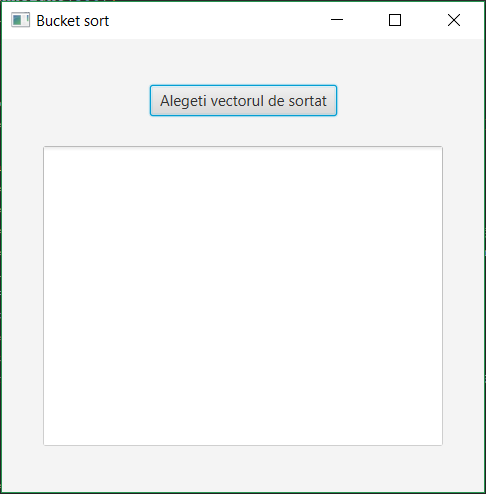
\includegraphics{aplicatie}\newline
După apăsarea butonului se deschide o fereastră de dialog care cere să se aleagă un fișier de tip text, care conține vectorul de sortat.\newline
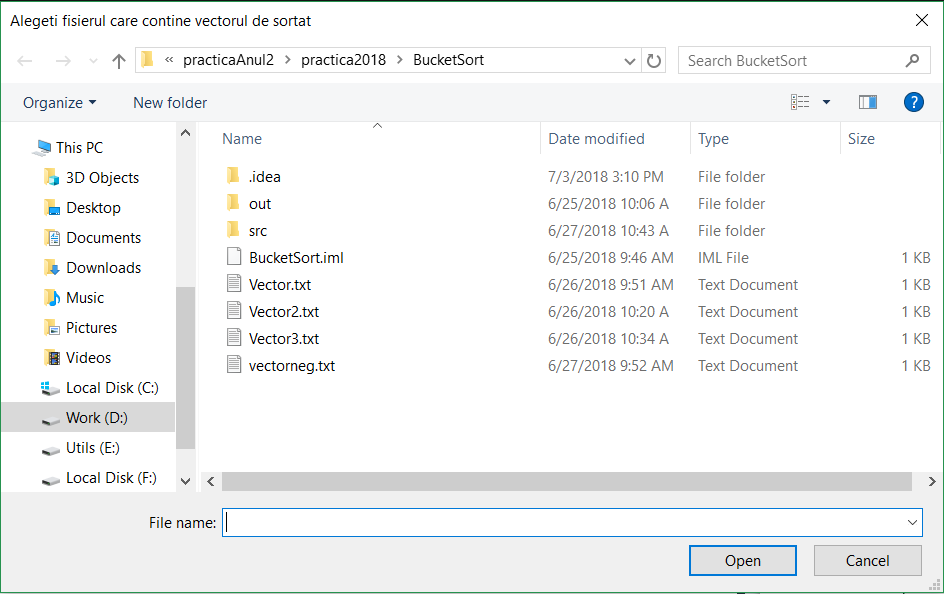
\includegraphics[scale=0.8]{fisier}\newline
După selectarea fișierului,care conține vectorul de sortat, se afișează în textarea vectorul din fișier si vectorul sortat.\newline
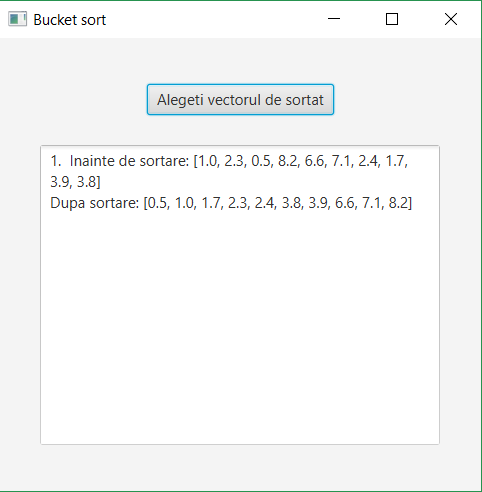
\includegraphics{sortat}
\section{Codul programului}
\subsection{Codul algoritmului}
\lstinputlisting[title=BucketSort.java ]{./BucketSort/src/BucketSort.java}
\subsection{Codul interfetei}
\lstinputlisting[title=Interfața.java ]{./BucketSort/src/Interfata.java}


\end{document}